
Most climate applications today read and write from and to parallel file systems such as Lustre.
The section describes how a POSIX-like backend to the ESDM would handle read and write requests and organise the ESDM data structures.


%%%%%%%%%%%%%%%%%%%%%%%%%%%%%%%%%%%%%%%%%%%%%%
\subsection{Logical View}
\label{backend: posix/logical}

\begin{figure}
	\centering
	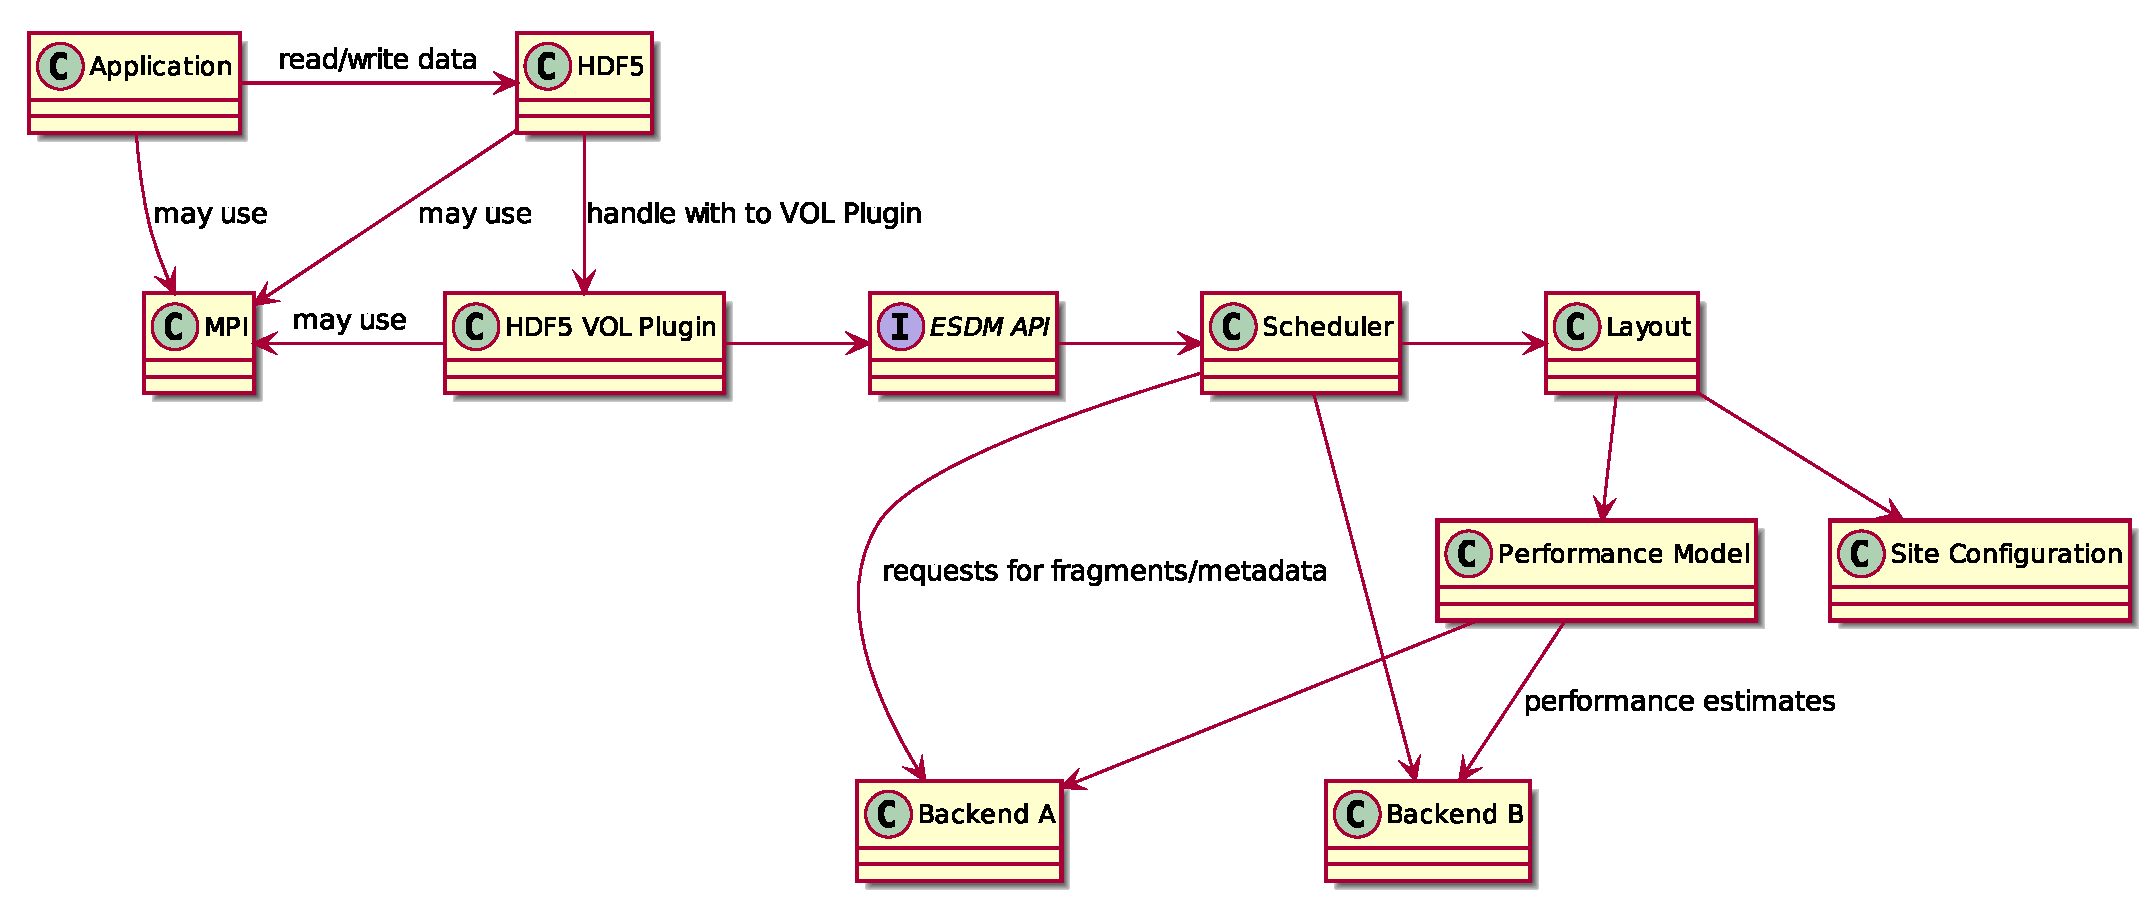
\includegraphics[width=\linewidth]{esdm-backends/POSIX/logical.eps}
	\caption{Logical view to the POSIX backend. I/O requests arrive through the ESDM API. The layout component provides a fragmentation (write: site config + perf model / read: as stored in metadata + optimisation candidate). As a result actual I/O requests are processed by the progress component which calls the backends. The backends and the datatype components work together to convert data according to what is required (again and read and write differ).}
	\label{fig:backend posix logical view}
\end{figure}

In the previous sections we have discussed how the scheduler (see \Cref{component: scheduler}) accepts requests by applications and libraries and then consults the layout component (\Cref{component: layout}) to decide on a layout.
In this section we assume the POSIX backend was chosen.
\Cref{fig:backend posix logical view} illustrates the involved components and which components interact with each other.
Requests made to the POSIX backend can be classified into one of three types.
On the one hand there are read and write requests to the data.
In addition, there maybe metadata lookup, which will in most cases relate to technical metadata.
The following paragraphs explain each of this access types in more detail.


\paragraph{Writing data}
To satisfy write requests this section extends the use-case description for general writing (see \Cref{uc: independent write}).
The sequence of events relevant to the POSIX backend (also illustrated in \Cref{fig:backend posix sequence write}) unfolds as follows:

\begin{enumerate}
	\item Progress: consults layout about:
	\begin{itemize}
		\item Which Backend?
		\item Which Fragmentation?
	\end{itemize}
	\item Scheduler: processes write calls for all fragments and hands data to POSIX backend
	\item Layout: decides for specific backend that is suitable for the individual fragment (e.g. row-way serialisation)
	\item Backend: converts between file serialisation and ESDM datatypes
\end{enumerate}

For a POSIX backend many potential mappings to files and directories are possible.
Which mappings are the most efficient is an open research question and depends on the application.
A straight forward approach is to use directory structure to map hierarchical concepts e.g. from NetCDF or HDF5 such as groups and data sets.
The files within data set directory would include a description of the domain and an additional directory that is used to store the actual fragments.

\begin{figure}
	\centering
	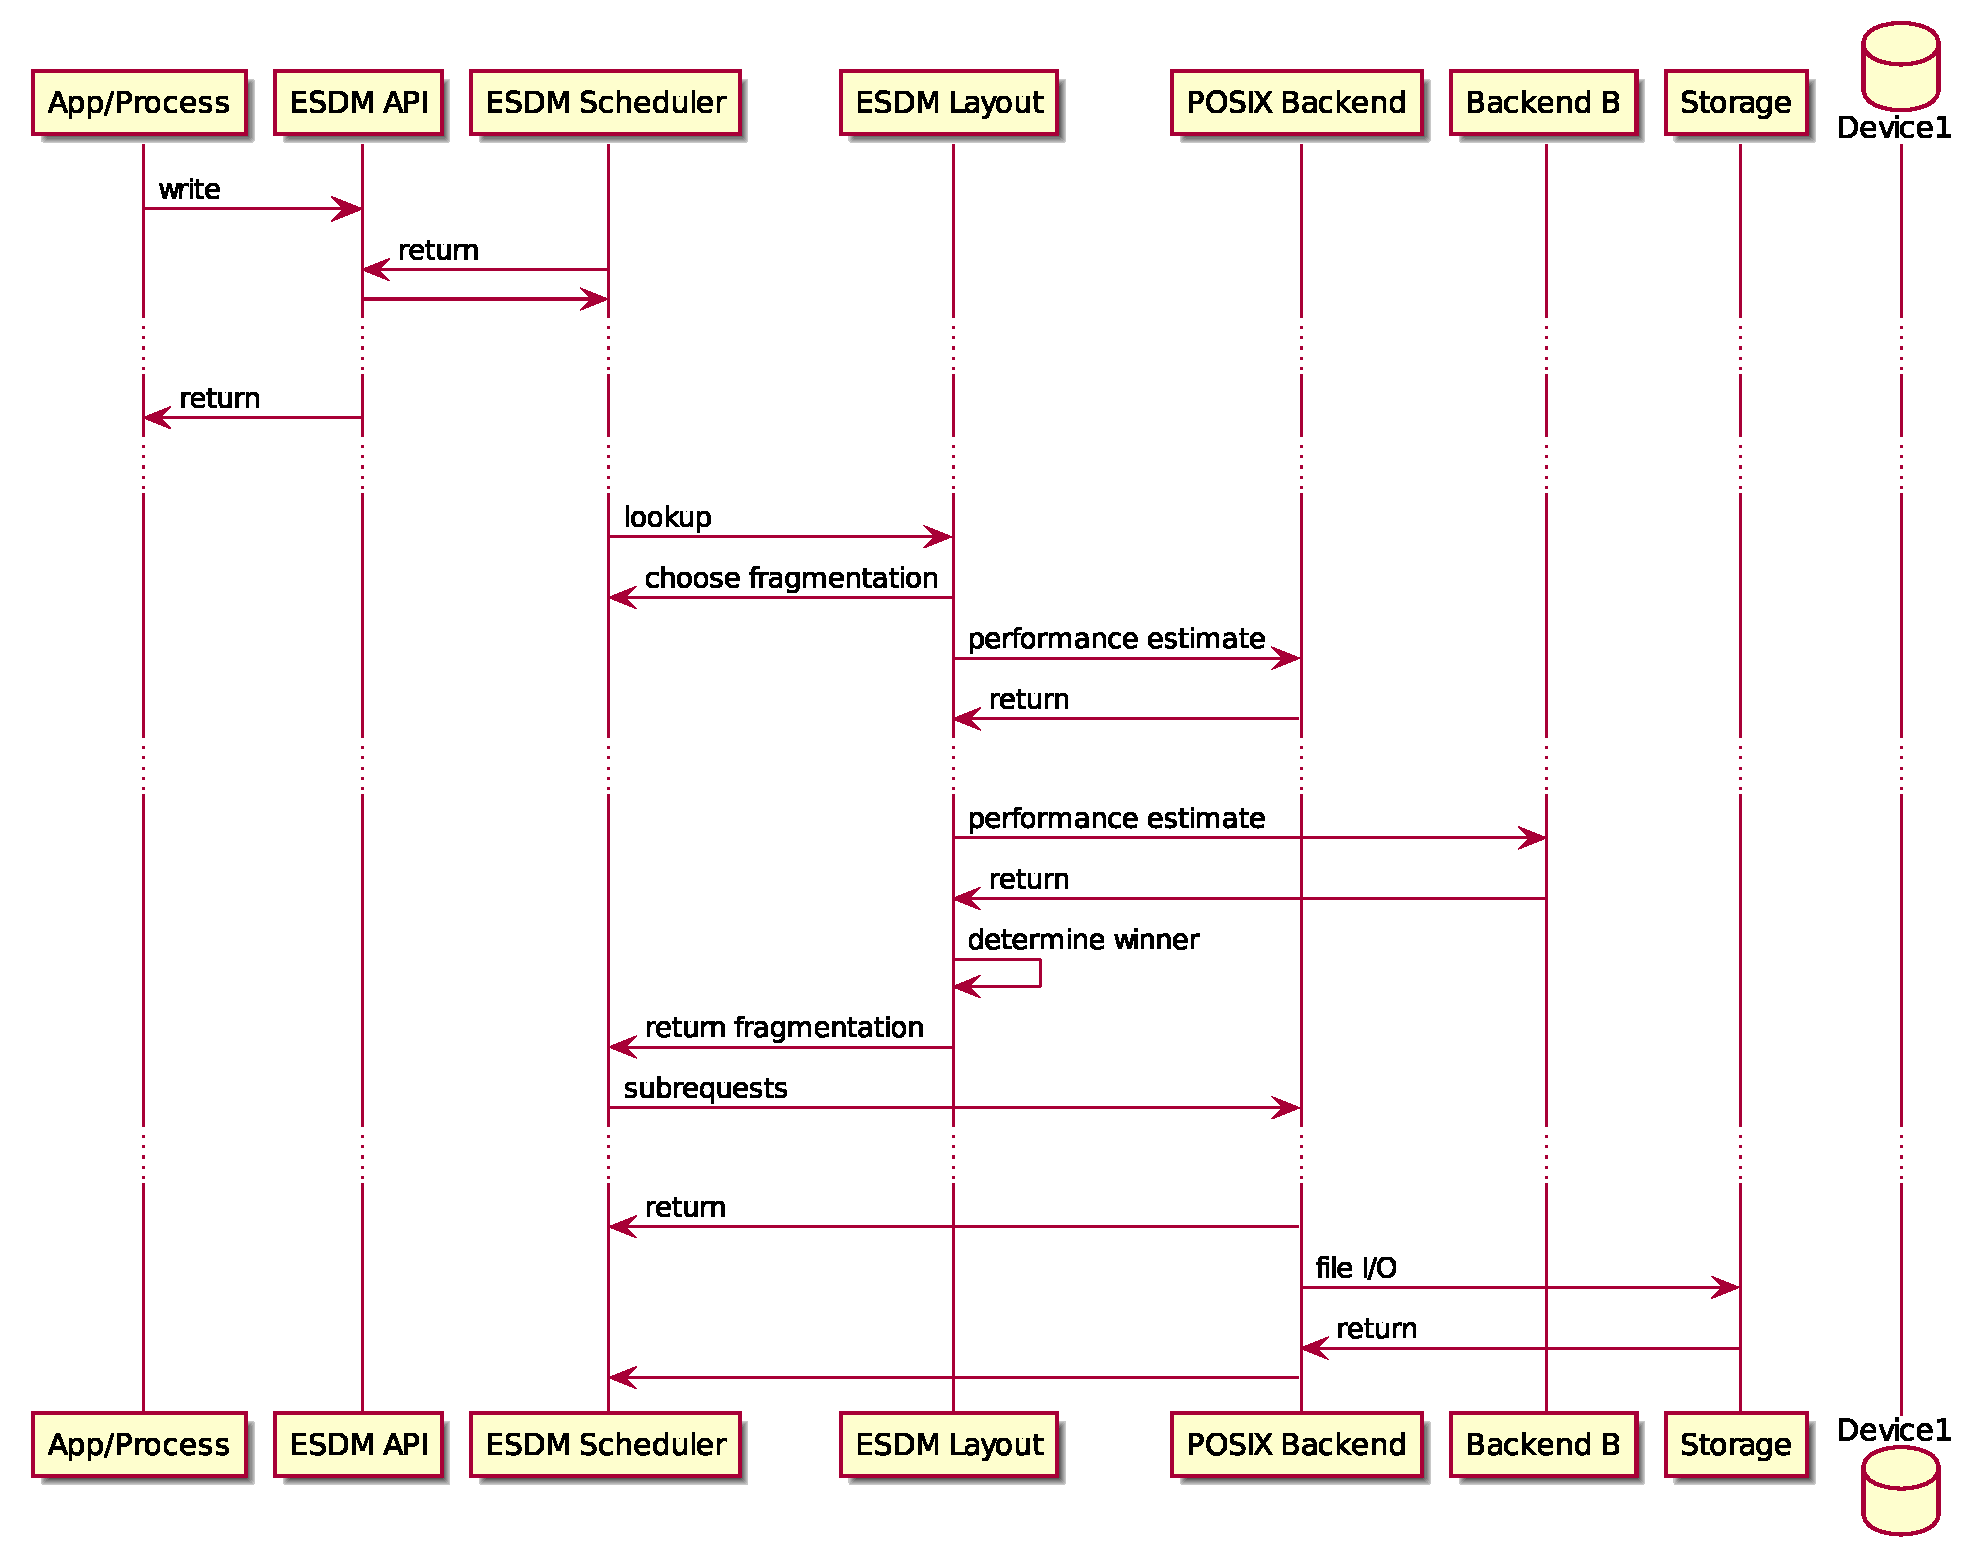
\includegraphics[width=\linewidth]{esdm-backends/POSIX/sequence_write.eps}
	\caption{Sequence Diagram for writes to the POSIX Backend.}
	\label{fig:backend posix sequence write}
\end{figure}



%%%%%%%%%%%%%%%%%%%%%%%%%%%%%%%%%%%%%%%%%%%%%%%%
\paragraph{Reading data}

Analogue to the write case, the reading data with a backend extends the use-case description for general reading (see \Cref{uc: independent read}).
The sequence of events relevant to the POSIX backend (also illustrated in \Cref{fig:backend posix sequence read}) unfolds as follows:

\begin{itemize}
	\item Read arrives
	\item Progress receives requests and splits it potentially into multiple sub requests
	\item Layout loads metadata, consults indexes and collects a sufficient amount of fragments to reconstruct requested (sub)domain in parallel and from the most ``affordable'' backends
	\item Progress (potentially coordinated across multiple processes) issues requests to backends
	\item Backends fetch data and return Fragments
	\item Backend + Layout + Datatype perform necessary conversations
	\item Data is provided to application
\end{itemize}



\begin{figure}
	\centering
	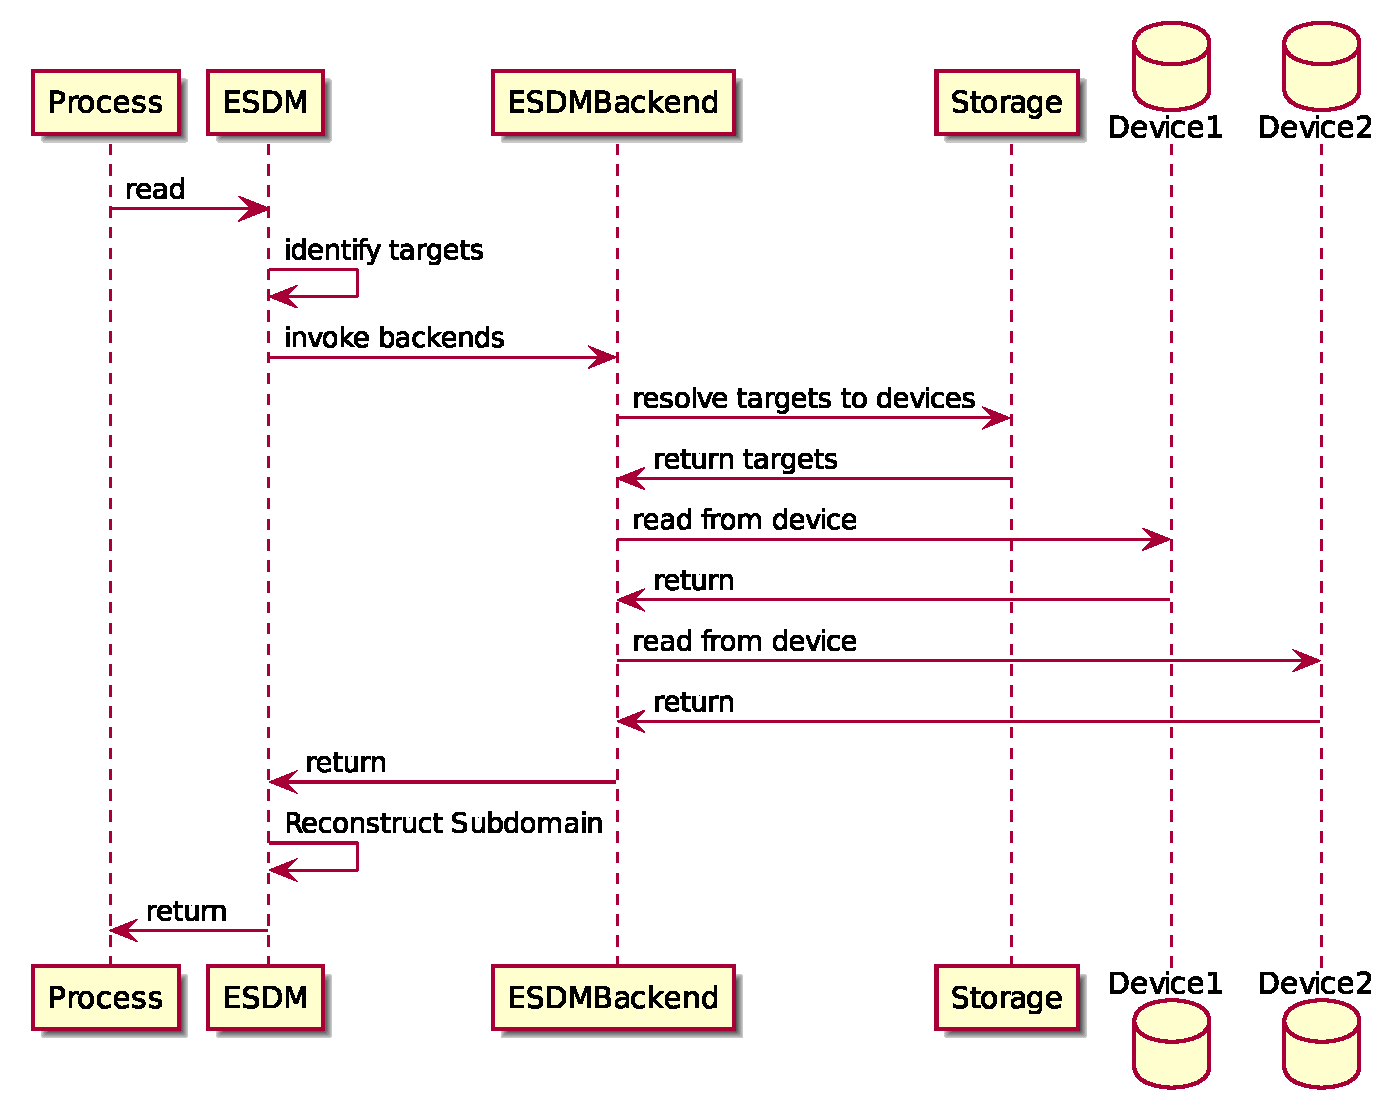
\includegraphics[width=\linewidth]{esdm-backends/POSIX/sequence_read.eps}
	\caption{Sequence diagram for reads to the POSIX backend.}
	\label{fig:backend posix sequence read}
\end{figure}



\paragraph{Lookup:}

\Cref{sec: viewpoints/logical/data model} introduced the ESDM data model.
A backend is responsible to store a fragment and find the fragment again when it is requested.
To allow for fast search for required fragments, the POSIX backend will use indexes.
In addition, fragments are written in sequence from a linked list that allows to reconstruct either the domain or or the index in case a index is damaged.
Fragments metadata should allow for partial access of fragment.
To allow this a POSIX Fragment wraps the ESDM fragment to attach technical metadata relevant only for the POSIX backend.
A UML diagram illustrating the relationship between POSIX Fragments and ESDM fragments is depicted in \Cref{fig:backend posix fragment}.

\begin{figure}
	\centering
	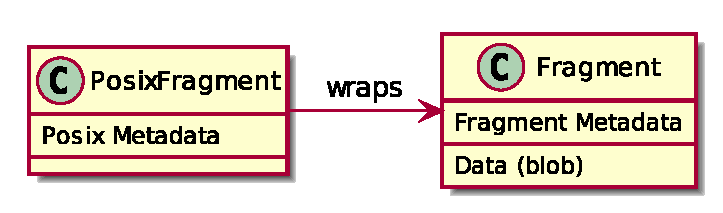
\includegraphics[width=0.5\linewidth]{esdm-backends/POSIX/fragment.eps}
	\caption{The ESDM Fragment features a Metadata section that describes the position within a domain. The actual data is simply a blob. Backends are free to extend ESDM Fragments to their liking.}
	\label{fig:backend posix fragment}
\end{figure}





%%%%%%%%%%%%%%%%%%%%%%%%%%%%%%%%%%%%%%%%%%%%%%
\subsection{Process View}
\label{backend: posix/process}

\begin{figure}
	\centering
	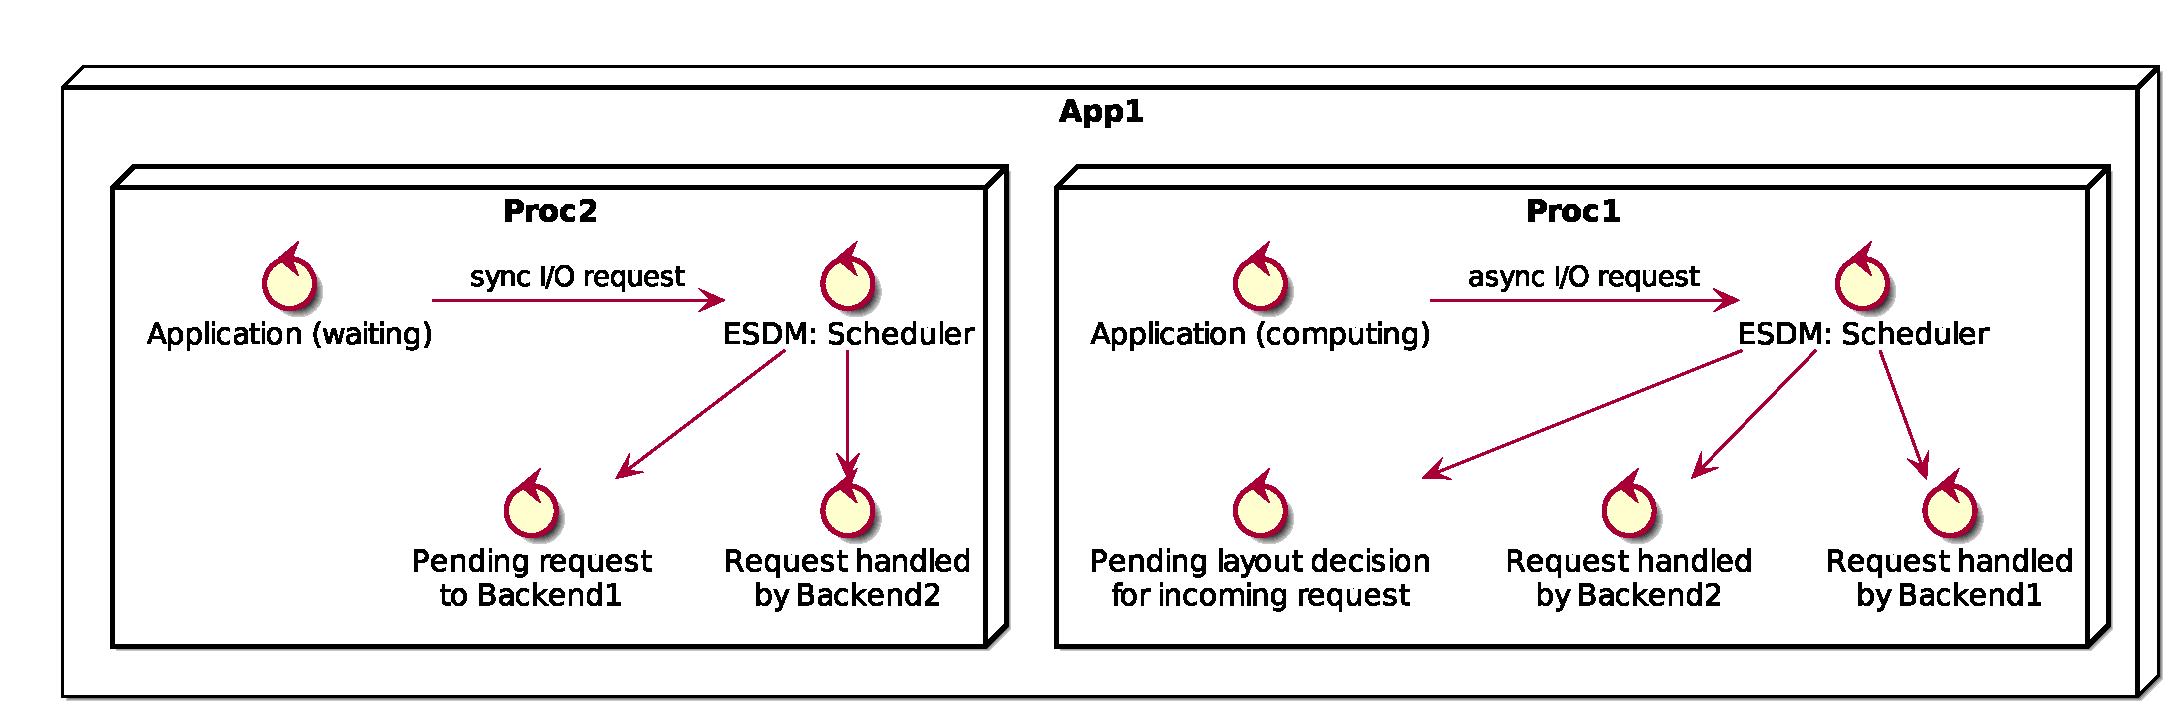
\includegraphics[width=\linewidth]{esdm-backends/POSIX/process.eps}
	\caption{Overview of processes that are necessary or interact/interfere with the POSIX backend.}
	\label{fig:backend posix process view}
\end{figure}

\Cref{fig:backend posix process view} illustrates the process view for the POSIX backend. In addition, interactions between the following services and processes are relevant:


\paragraph{Scheduler component}
The progress component is responsible for handling any sync calls as well as outstanding async calls that have to be passed to the backend.


\paragraph{ESDM Compactor component}
The ESDM compactor may either reorganise POSIX data snippets on their on.. e.g. when running as daemon that improves and maintains the system health.
As applications issue I/O the progress component may use the ESDM compactor when the decision component determines feasible reorganisation/compactification.


\paragraph{(Competing Load):}
Other resources may access the same storage backend, or even the same data.
For example workflows may compete for access to the same storage target.
This may influence the decisions used for compactification.


\paragraph{(Service Loads):}
The backends usually employ service workloads that ensure system health.
%How do ESDM and there workloads interfere with each other?




%%%%%%%%%%%%%%%%%%%%%%%%%%%%%%%%%%%%%%%%%%%%%%
\subsection{Physical View}

Active software components related to the ESDM that are involved in handling requests are spread across the application process and when they are finally written on the POSIX storage system as illustrated in \Cref{fig:backend posix physical view}.
No changes to POSIX are assumed, but a POSIX backend will call the interfaces these storage systems expose.

Notice that POSIX in this graphic provides a performance model, which is technically not the case for the current ESDM because the system runtime information such as fill level are not communicated actively by the storage system but are instead collected by, e.g., the ESDM POSIX Backend Plugin.


\begin{figure}
	\centering
	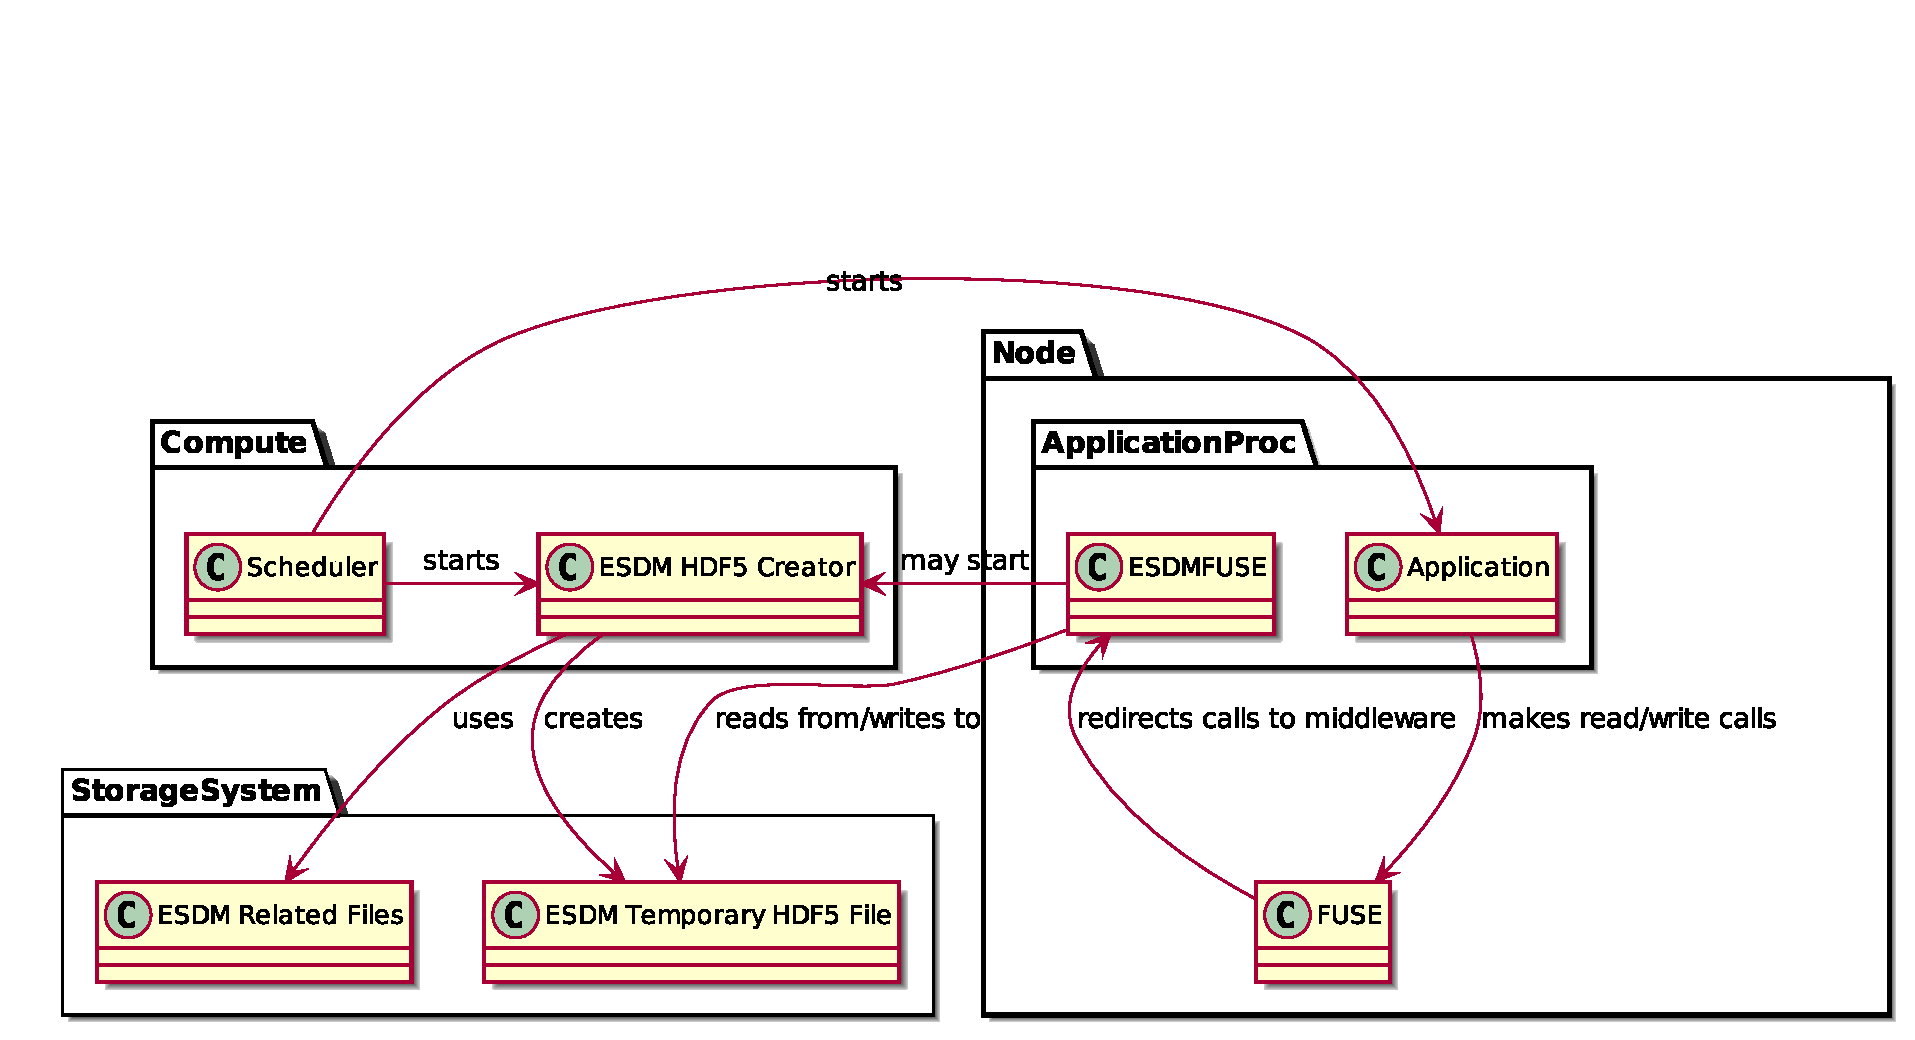
\includegraphics[width=\linewidth]{esdm-backends/POSIX/physical.eps}
	\caption{Physical mapping of components to location of their execution?}
	\label{fig:backend posix physical view}
\end{figure}



%%%%%%%%%%%%%%%%%%%%%%%%%%%%%%%%%%%%%%%%%%%%%%%
%\section{PFS Backend}
%
%\todo{Relocate into Architecture Section?}
%\todo{Probably multiple such use cases to describe the backends.}
%
%Storage entities: files, directories
%
%Permissions:
%* Mapping description
%
%Mapping from containers, variables and fragments:
%A fragment is a file:
%* data
%* support structures (index)
%
%Epoch
%*
%
%
%General description of PFS backend. Motivated by use cases.
%
%
